%!TEX root = batch-course.tex
%-------------------------------------------------
\section{Case study: Granulator process}
%-------------------------------------------------

\begin{frame}\frametitle{GSK granulator case study: background}
	
	\begin{columns}[t]
		\column{0.5\textwidth}
			\( N = 14 \): one problematic batch
			{\scriptsize
			\begin{enumerate}
				\item 		  317655
				\item		  319341
				\item		  319340
				\item		  319339
				\item		  319336
				\item		  319334
				\item		  319333
				\item		  317649
				\item		  317648
				\item		  317647
				\item		  315876
				\item		  315875
				\item		  315874
				\item		  319343
			\end{enumerate}
			}
			
		\column{0.5\textwidth}
				\( K = 8 \) tags:
				\begin{itemize}
					\item	Chopper current
					\item	Chopper speed
					\item	Impeller speed
					\item	Impeller current
					\item	Impeller Watts
					\item	Product temperature
					\item	Solvent vessel air pressure
					\item	Spray solution flowrate
				\end{itemize}
	\end{columns}
\end{frame}

\begin{frame}\frametitle{GSK granulator case study: loadings}
	
	\begin{itemize}
		\item	Score plot
	\end{itemize}
	\begin{center}
		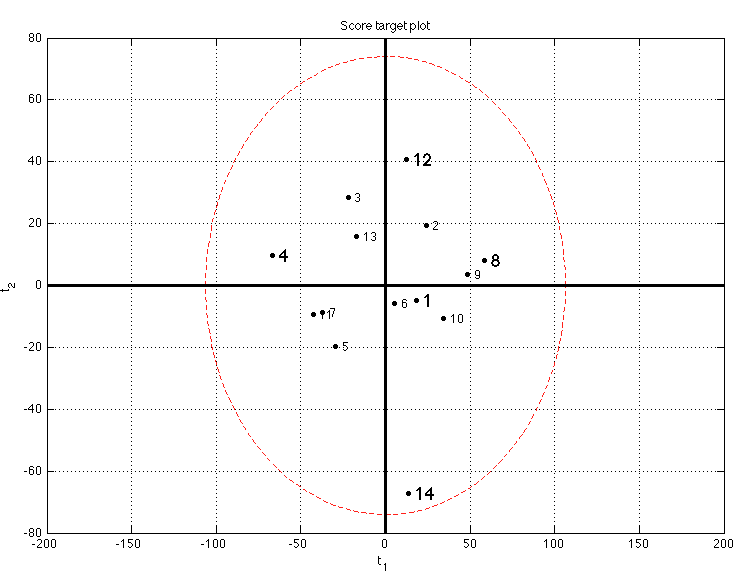
\includegraphics[width=0.8\textwidth]{images/gsk/GSK-score-plot.png}
	\end{center}
	
\end{frame}

\begin{frame}\frametitle{GSK granulator case study: loadings}
	
	\begin{itemize}
		\item	Loadings: \( p_1  \) and \( p_2 \)
	\end{itemize}
	\begin{center}
		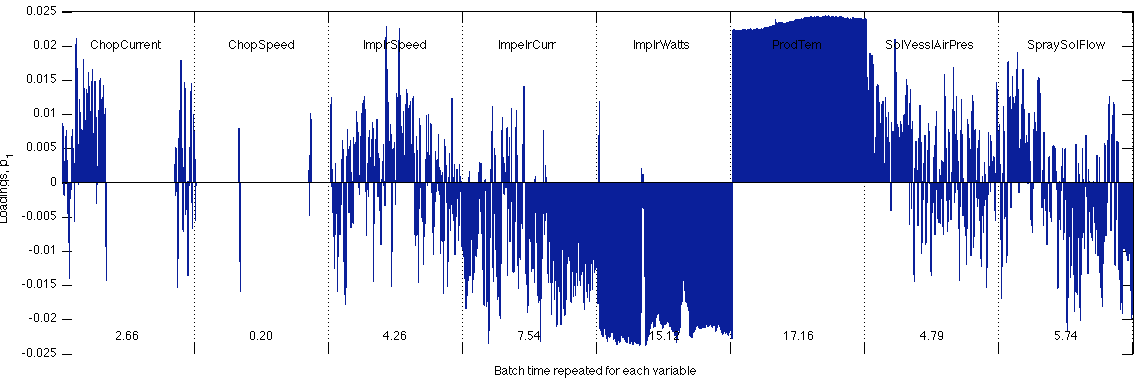
\includegraphics[width=\textwidth]{images/gsk/GSK-loadings-p1.png}
	\end{center}
	\begin{center}
		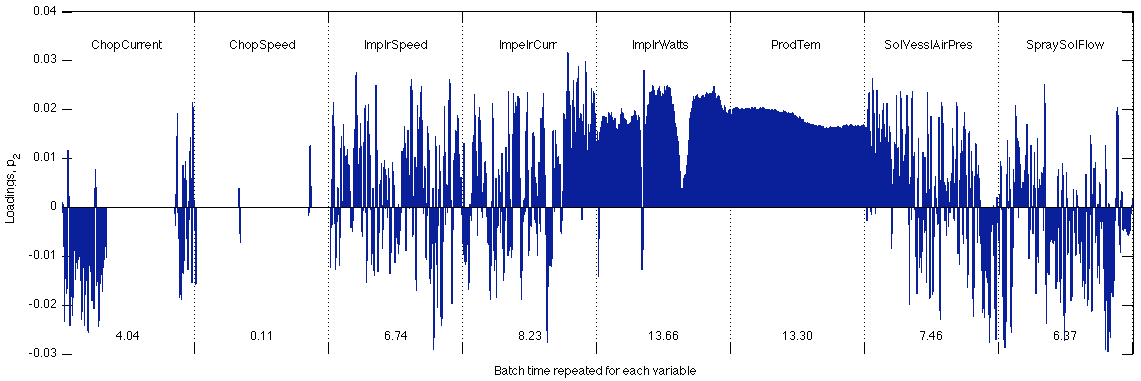
\includegraphics[width=\textwidth]{images/gsk/GSK-loadings-p2.png}
	\end{center}
\end{frame}

\begin{frame}\frametitle{GSK granulator case study: \( R^2 \)}

	\begin{center}
		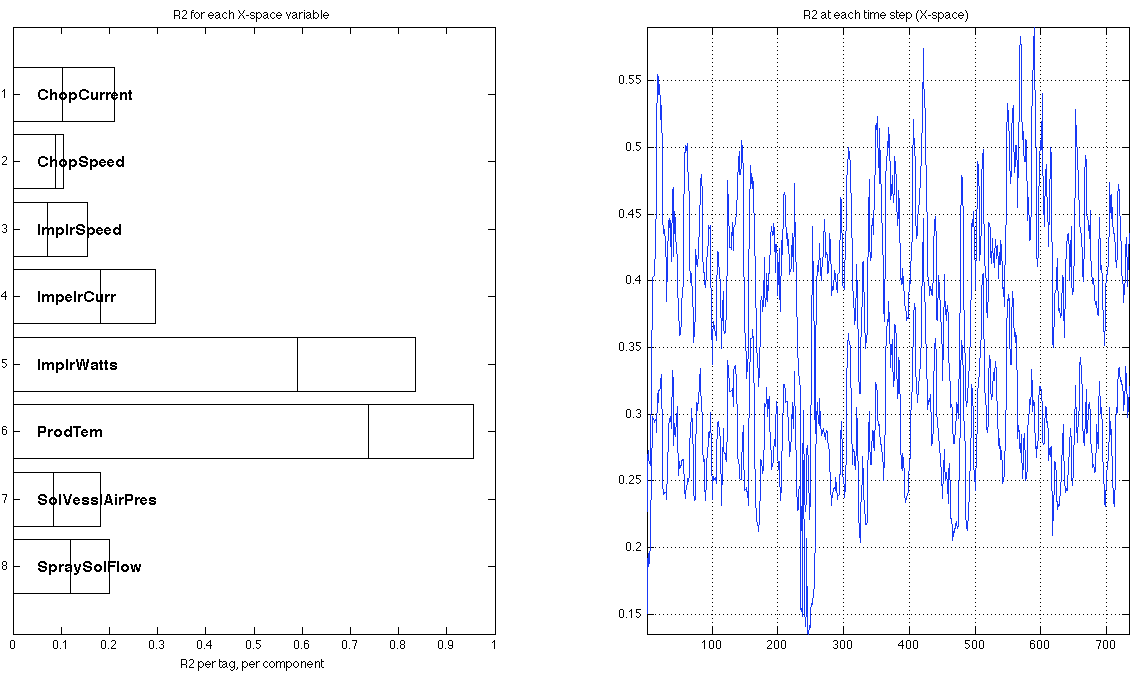
\includegraphics[width=\textwidth]{images/gsk/GSK-R2-plot.png}
	\end{center}

\end{frame}


